\section{The Vignetting Model}

\subsection{Why Ghosting Alone Is Not Enough}

The ghost formula above assumes we already know \emph{which pairs of holes}
are simultaneously letting light through to the eye. When the eye looks
straight ahead, the pupil sits centered behind the array, and it is easy to
list which holes fall under it. But the pupil is a physical opening of fixed
size, and the eye rotates constantly during normal viewing. As it rotates,
the pupil's position relative to the fixed hole pattern shifts --- some
holes that were fully under the pupil become partially or fully blocked,
and others that were outside the pupil's reach can come into play.

\intuitbox{This means a design that looks perfectly safe --- even \emph{trivially}
safe, with no two holes ever simultaneously active --- when evaluated only
at straight-ahead gaze can become unsafe the instant the eye looks even a
little to one side. You cannot conclude a design is safe from the
straight-ahead case alone; you have to check across the whole range of
gaze angles a person actually uses.
}
\subsection{The Geometry}

The pupil and a given hole are both circles. As the eye rotates by an angle
$\varphi$, the pupil's center shifts laterally relative to the hole pattern
by approximately
\begin{equation}
\Delta(\varphi) \approx R_{\rm rot} \sin\varphi
\end{equation}
where $R_{\rm rot}$ is the eye's physiological rotation radius
($\approx$13--14mm). The overlapping area between the pupil (radius
$R_p$) and a hole (radius $R_h$), once their centers are separated by
$\Delta$, is the standard geometric formula for the overlap of two circles:
\begin{equation}
A_{\rm overlap}(\Delta) = R_p^2\cos^{-1}\!\left(\frac{\Delta^2+R_p^2-R_h^2}{2\Delta R_p}\right)
+ R_h^2\cos^{-1}\!\left(\frac{\Delta^2+R_h^2-R_p^2}{2\Delta R_h}\right)
- \tfrac12\sqrt{(-\Delta{+}R_p{+}R_h)(\Delta{+}R_p{-}R_h)(\Delta{+}R_h{-}R_p)(\Delta{+}R_p{+}R_h)}
\end{equation}
with two edge cases handled separately: if the circles no longer touch at
all ($\Delta \ge R_p+R_h$), the overlap is exactly zero; if one circle sits
entirely inside the other ($\Delta \le |R_p-R_h|$), the overlap is simply
the area of the smaller circle. A na\"ive implementation of the general
formula can return a tiny negative number right at this second boundary,
purely from floating-point rounding --- a real bug this project found and
fixed by explicitly clamping the result to zero at the boundary.

\subsection{How the Implementation Was Checked}

The closed-form formula above was tested against a second, completely
independent method: randomly scatter thousands of points inside a hole's
area and simply count what fraction land inside the shifted pupil circle
(a Monte Carlo estimate). If the two methods --- one algebraic, one
brute-force random sampling --- agree, that is strong evidence the formula
was implemented correctly, since the two approaches share no code and could
not fail in the same way by coincidence. Figure~\ref{fig:vignvalid} shows
this comparison, converging to under 0.2 percentage points of relative
error.

\begin{figure}[h]
\centering
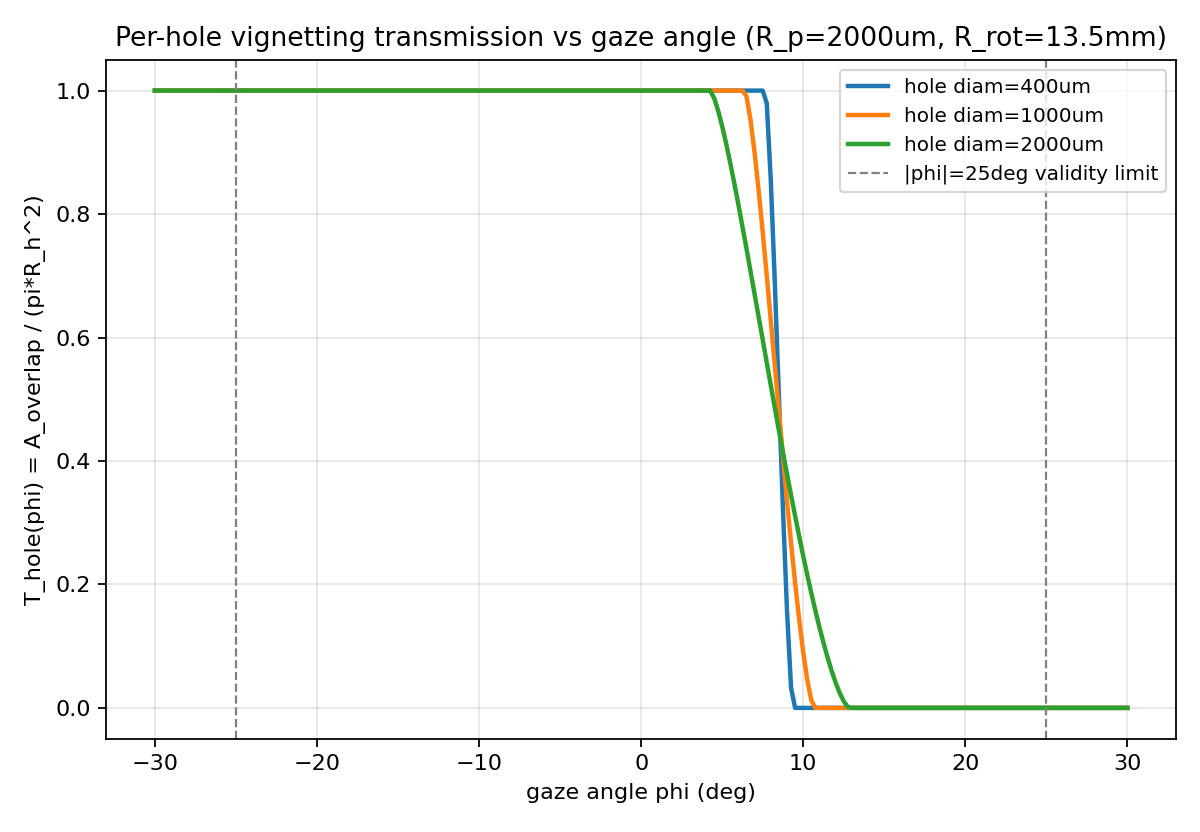
\includegraphics[width=0.85\textwidth]{handbook_figs/vignetting_validation.png}
\caption{Closed-form overlap-area formula versus an independent Monte Carlo
estimate, across gaze angle $\varphi$. Agreement here is what justifies
trusting the fast closed-form version for large sweeps instead of running
the (much slower) random-sampling method every time.}
\label{fig:vignvalid}
\end{figure}

\codemapbox{This geometry lives in \texttt{array\_optimization/vignetting.py}
(the original, validated implementation) and is copied into
\texttt{array\_geometry\_lab/degeneracy\_filter.py}\footnote{Copied rather
than imported for the large sweep pipeline, for speed --- but re-checked
byte-for-byte against the original's own validation data before use, so the
copy could not silently drift from the original.} for fast repeated use
across the geometry-comparison sweep. The safety rule built on it,
\texttt{gate\_vignetting\_safety()} in \texttt{comparison\_metric/gates.py},
re-runs the ``which holes are active'' calculation at many gaze angles
(0\textdegree\ to $\pm$25\textdegree) and requires the design to stay
ghost-safe at \emph{every} one of them, not just at $\varphi=0$.
}
\newpage
